Before getting to all the fun graphs, we will need to introduce some concepts, so you\footnote{yes, \textit{you} specifically} can follow along while keeping me somewhat consistent with the literature:

\begin{enumerate}
    \item Upper/Lower $\rightarrow$ Dorsal/Ventral
    \item Front/Back  $\rightarrow$ Anterior/Posterior
    \item   $\rightarrow$
\end{enumerate}

Whenever a diagram or image of the egg is show, the Anterior side is pointing to the left.

\section{Broken Symmetries and Genetic Patterning}
% \section{Everything}
\label{sec:theory-polarity}
\subsection{Broken Symmetries}

Almost all animals [Citation needed] start as a single, isotropic sphere of epithelial cells. At one point, this ball will 'turn in on itself' and begin developing the basis for organogenesis. This process is called gastrulation. As animals are not spherically symmetric\footnote{except for your mom}, a number of symmetries need to be broken. 

In drosophila, after the first rounds of mitosis, the cells migrate to line the inside of their egg. This allows their surfaces form distinct "outside" and "inside" domains. Through preferential adhesion\footnote{explain  preferential adhesion} based on their individual surface orientation, the cells can maintain the shell-form, thereby giving rise to the well-defined Inside-Outisde polarity. In biology this is known as Apical-Basal polarity (AB-polarity from here on) and is seen in almost every multicellular system. 





Diffusion based concentration gradients along with the aforementioned polarities allow for spatially complex, precise and robust macro scale morphology changes.

\subsection{Genetic Patterning}
\label{sec:gen_patterns}
All multicellular organisms, will need to go from a simple single cell to forming the complex body plans we all know and love. This complicated interplay between cells will needs organization. Again, for humans and fruit fly alike, this is done via genetic patterning.\cite{veraksa2000developmental}

As predicted by Turing, the patterning is a result of "smartly"\footnote{I know, I know, Nature abhors a vacuous anthropomorphization} designed catalyzing or inhibiting chemical interactions. But thinking about it top-down is inaccurate. A lot of the concentrations are directly impacted by by the cells themselves. 


% Now, to shake it up, \textit{Twist} \& \textit{Snail}, which might remind you of the beetles,\footnote{The species \textit{Tribozium} for example\cite{sommer1994expression}} are vital for the early development of a surviving fruit fly.


During the development of our model, the data and resources at \url{https://shiny.mdc-berlin.de/DVEX/} have been absolutely vital.

TODO: Maybe explain data-processing?

This allowed us making maps. Where we initially defined areas of interes after hand-drawn cell-fate maps, we can now specify boundaries between cell types on the unperturbed morphology using interactions between maternal gradients. A selection fo some of the most vital morphogens can be seen in tabek \ref{tab:morphogens} and in Figure \ref{fig:MorphogenMap} their concentrations can be seen as mapped onto our virtual blastoderm.


\begin{table}[H]
\begin{tabular}{lll}
 \begin{tabular}[c]{@{}l@{}}Genetically patterned \\ transcription factor proteins\end{tabular} & Location at gastrulation & Vital for development of \\ \hline
 Twist \& Snail                                                                                 & Ventral                  & Mesoderm                 \\
Huckebein \& Tailless                                                                          & Posterior                & Endoderm (Midgut)   \\

 Runt \& Even skipped & Germ Band & All of the above\\
Buttonhead \& Even skipped  & Cephalic furrow & Chephalic furrow\\

\end{tabular}
    \caption{The most important morphogens and their simplified reason of significance}
    \label{tab:morphogens}
\end{table}


\noindent

\begin{figure}[H]
    \centering
    \makebox[\linewidth]{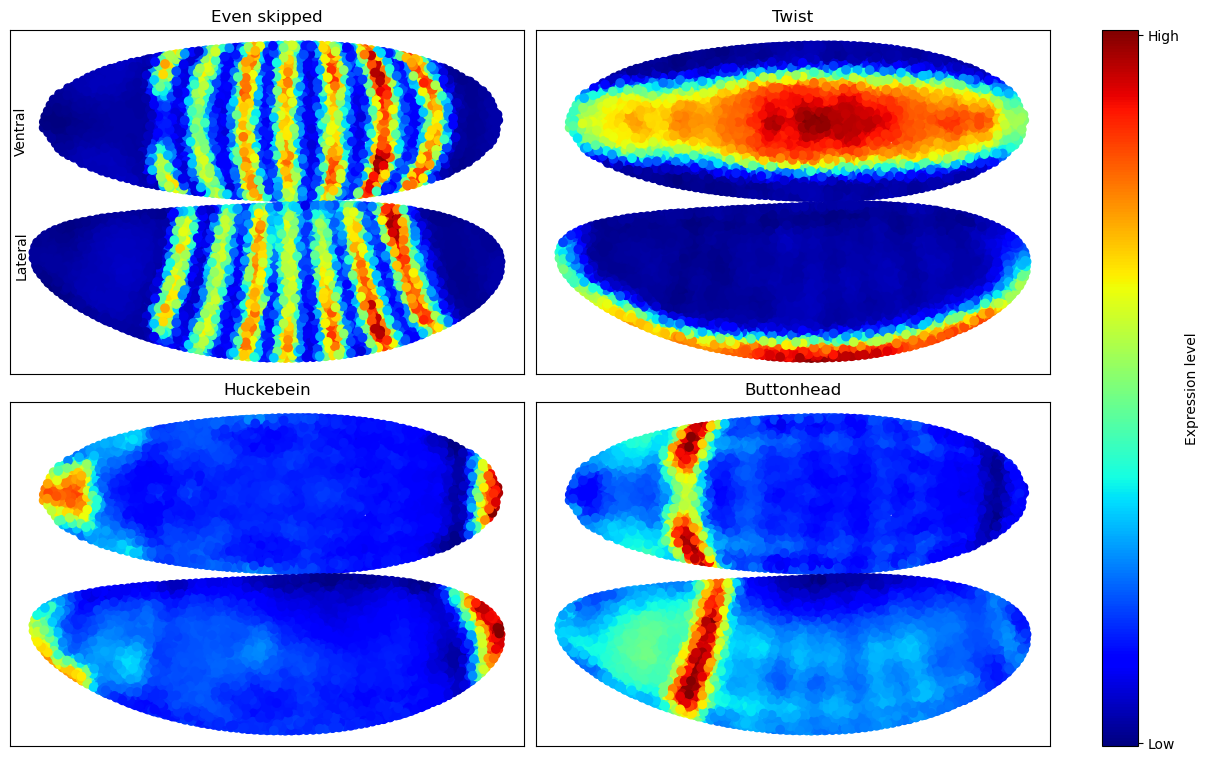
\includegraphics[width=1.2\linewidth]{chapters/Theory/figures/patterning.png}}
    \caption{The data extracted from \url{https://shiny.mdc-berlin.de/DVEX/} as projected onto our embryo. A clear attest to the remarkable and stable pattern formation Turing predicted chemicals gradients capable of producing.}
    \label{fig:MorphogenMap}
\end{figure}

Importantly, the interaction between the morphogens and the mechanical deformations go both ways. It has been shown (J. Schauser et al) that a mechanical stimulus can trigger a chemical signal, thereby reinducing patterning in a feedback loop. This is called mechanotransduction and is believed to be vital in stable PCP-orientation. [citation needed]


\textbf{Important:}
The PCP has been shown to be gradient of striping


\section{How cells move}

In general, most of the global large-scale cell migration seen during development of multicellular organisms stem from a handful of seemingly simple\footnote{albeit still not well understood} active single-cell actions.\cite{walck2014cell}\\
The cells internal structure is called the cytoskeleton with internal \textit{motor proteins} responsible for keeping and changing the cells shape.

The motion we will be looking at, are of a type that is fundamentally different from Chemotaxis, with cells reacting to a local chemical concentration but not moving along a gradient [citation needed]. The global changes in physical structure we will be exploring all arise from cell actions with little to no discernible individual movement.


When we talk about the individual cells, this is a simplification. As can be seen on Figure \ref{fig:mysosinMeshwork}, the cells stay interconnected using membrane tethers connecting local neighborhoods. 

\begin{figure}[H]
    \centering
    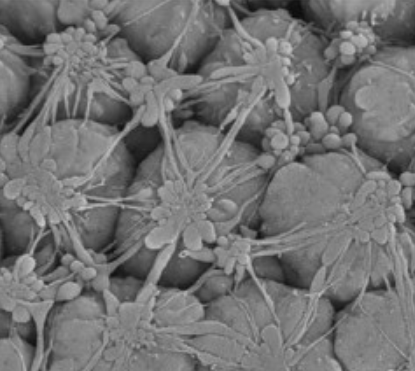
\includegraphics[width=0.6\linewidth]{chapters/Theory/figures/EM_constricting_proteins.png}
    \caption{Electron microscopy of Myosin II meshwork at ventral side. Taken from \cite{martin2010integration}}
    \label{fig:mysosinMeshwork}
\end{figure}

In Drosophila gastrulation, the role of these 'driving effects' are surprisingly under-understood with no paper claiming YYY with certainty.\footnote{This very much comes down to the fact, that experiments with living, moving cells are inherently intractable/hard} Here is a list of the fundamental single-cell active forces that is undeniably happening, even if not essential for the final outcome:\footnote{As nature is remarkably resilient, there is clear and definite evidence of one action overtaking when another fails to deliver. \textbf{Rewrite} This will be expanded upon in Section \ref{sec:mutantNoGB}} 

\subsection{Convergent Extension}
For elongating the germ band Convergent Extension seems to be the main proprietor of movement. Consisting of asymmetric cellular intercolations, tissue can change shape without the individual constituents looking any different.  

\begin{figure}[H]
    \centering
    \begin{subfigure}{0.45\linewidth}
        \centering
    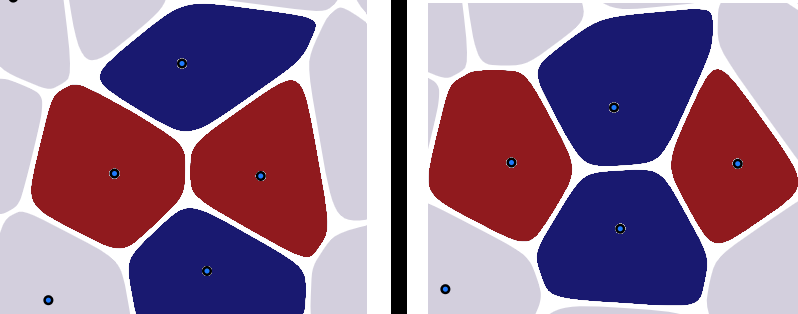
\includegraphics[width=\linewidth]{chapters/Theory/figures/ConvergentExtensionDiagram.png}
    \caption{A diagram showing how guided intercolation results in directional elongation}
    \end{subfigure}
        \begin{subfigure}{0.45\linewidth}
        \centering
        \caption{Dyed Germ Band tissue showing clear difference in horizontal and vertical protein expressions}
    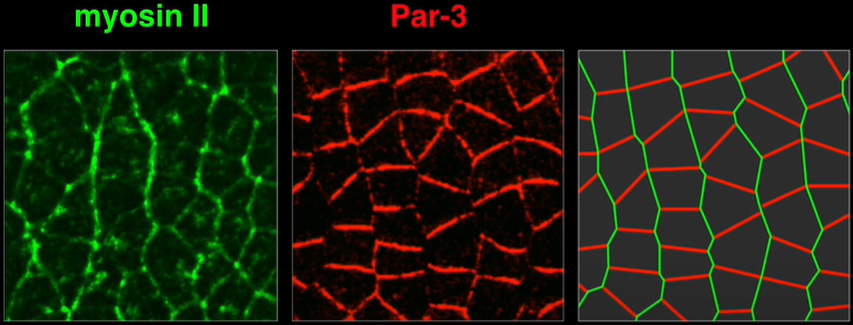
\includegraphics[width=\linewidth]{chapters/Theory/figures/bipolar-PCP.png}
    \end{subfigure}
    \caption{\cite{zallen2004patterned}\url{https://www.youtube.com/watch?v=MO7x7R-m3Qk}}
    
    \label{fig:ConvergentExtensionDiagram}
\end{figure}

Wieshaus and [hende damen der] showed through laser ablation, Cell Intecolation. Anisotropic constriction of cell borders with deformations only happening  



We know that the signaling protein Wnt plays an important role in controlling Convergent Extension. For interesting writing, here is some foreshadowing: Wnt is also known as an inducer of Planar-Cell-Polarity.

\subsection{ Apical Constriction }
When the cell sheet wants out-of-plane bending, they turn to Apical Constriction. Apical constriction functions exactly as you would think; Myosin rings constrict the apical (outer) side of the cell, creating a smaller surface area. This leads to bending and, when enough constriction is applied, invagination. (see Figure \ref{fig:apical-constriction}). Cells has been shown the ability to constrict both isotropically and anisotropically.

\begin{figure}[H]
    \centering
    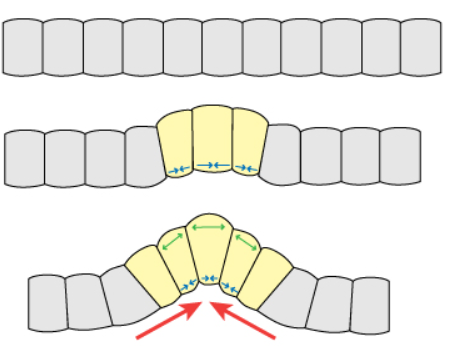
\includegraphics[width=0.3\linewidth]{chapters/Theory/figures/apical_constriction_schematic.png}
    \caption{Schematic for how apical constriction works}
    \label{fig:apical-constriction}
\end{figure}


\subsection{Cell Shape Change}
At the onset of gastrulation, the cells are tightly packed, giving them a pronounced elongated shape. As their apical and basal sides are smaller, the cells can use their cytoskeleton to actively reshape their volume in plane quite drastically. 

\subsection{Proliferation}
If cells are dividing in-plane, they can apply a pressure. In the stages of we are looking at, cell-division is shown to not be a driving force.

\section{Drosophila in detail}
\subsection{The Drosophila Embryo in detail}
\label{sec:drosophila-embryo-detail} 
We will quickly outline the main morphological features of the gastrulation cycle of the embryo:
\begin{outline}
    \1 Posterior Midgut (PMG)
    \1 Anterior Midgut (AMG)
    \1 Ventral Furrow
    \1 Dorsal Transverse Furrows
    \1 Cephalic Furrow
    \1 Germ Band
\end{outline}

\begin{figure}[H]
    \centering
    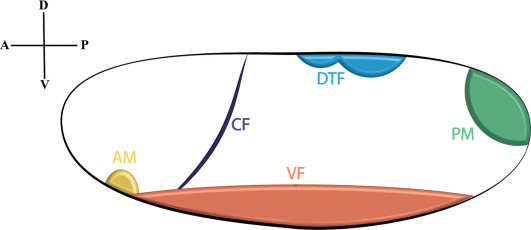
\includegraphics[width = 0.7\linewidth]{chapters/Theory/figures/morphogenic_events.jpg}
    \caption{Summary of the morphogenetic events mapped onto the blastoderm stage embryo. Taken from \cite{gheisari2020gastrulation}. The colored parts are generally seen to be the morphogenetically active during the early part of the embryogenesis}
    \label{fig:enter-label}
\end{figure}

IN OUR SIMULATION: 

The Germ Band is defined as all cells expressing a sufficient YY of the two striped genes \textit{Eve} and \textit{Run} the at the onset of gastrulation. \cite{zallen2004patterned}
\subsection{The Drosophila Gastrulation in detail}
Now, with the details in place, we can get to the main event!
In 1975 Bownes et al. split the development of the fruit fly from fertilised egg to hatched larvae into 17 distinct events. \cite{bownes1975photographic} We will be looking at stages 5 through 7, lasting about 15 minutes. These are characterized by having the first mesoscopic morphogenetic movements and setting the stage for all the morphology to come. 

The Drosophila morphogenesis consist of a series of interconnected localized cell movements. I will here present an abridged (The "Good Parts" Version) overview, roughly ordered in time:
\newpage

\begin{figure}[H]
    \centering
    \vspace*{-1cm}\makebox[\textwidth]{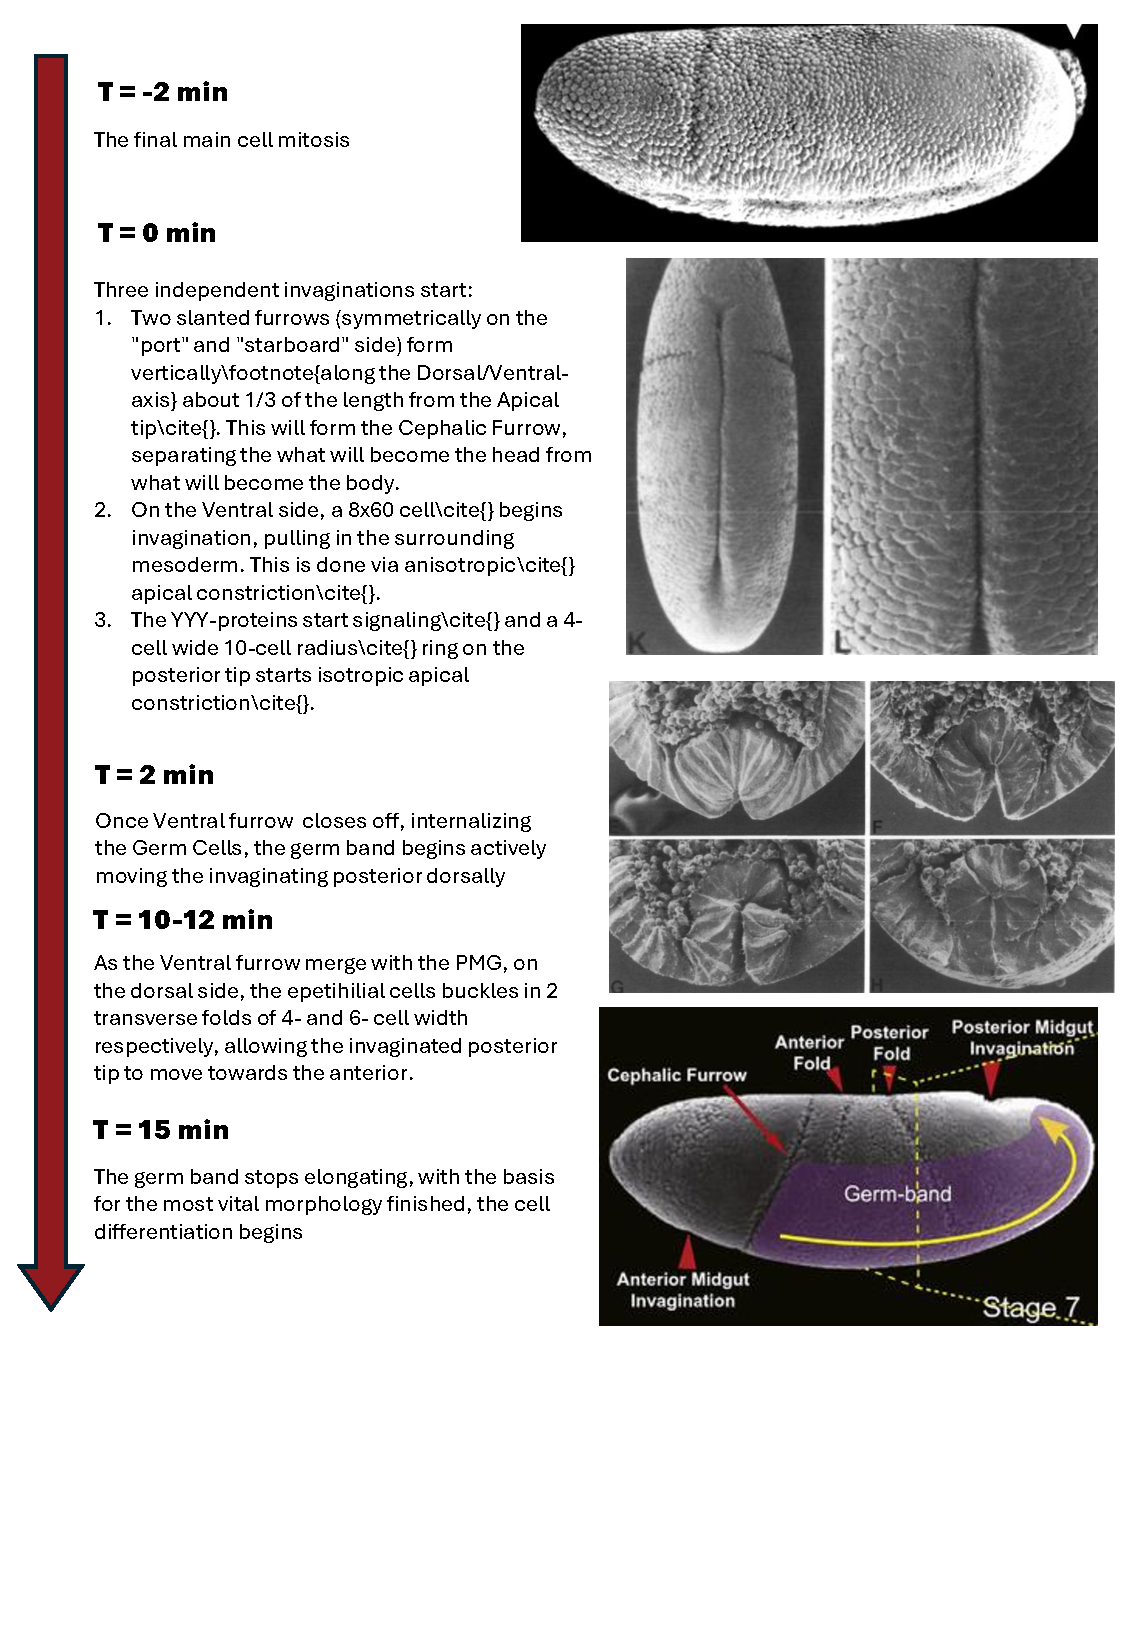
\includegraphics[width=0.8\paperwidth]{chapters/Theory/figures/Timeline.pdf}}
    \caption{Caption}
    \label{fig:big-timeline}
\end{figure}
\newpage
\addtocounter{figure}{-1}
\begin{figure} [t!]
  \caption{(Previous page.) \\ A somewhat comprehensive explanations of the most important past of the initial parts of the gastrulation.
  }
\end{figure}
\section{Previous attempts at simulation?}
While in silico models has provided multiple working examples of all the aforementioned embryogenesis events, their interplay has proven hard to study.

Mainly finite-element simulations have dominated the field when studying the physics of tubologenesis, tissue-folding etc.  

This all leads us to the star of the show:

\section{The Model}
The model is built around simply simulating the movement of the center of mass of the cells along with their individual orientation. 

As described in \cite{} and \cite{}, the model is based on the following intercellular potential:

\begin{equation}
    V_{ij}=e^{-r_{ij}}-A_{ij}e^{-r_{ij}/\beta}
\end{equation}

Where the individual cell wants to minimize the quantity 
\begin{equation}
    U_i = \sum_j V_{ij}
\end{equation}
Here the sum over $j$ is over all Line of sight/Voronoi neighbors (biologically founded if you remember the nearest neighbor protein connections in Figure \ref{fig:mysosinMeshwork}). 


For $A_{ij}=1$ (we will soon expand on this term), the potential simply looks akin to a Yukawa/YYY potential and can be seen in Figure \ref{fig:potential} 
\begin{figure}[H]
    \centering
    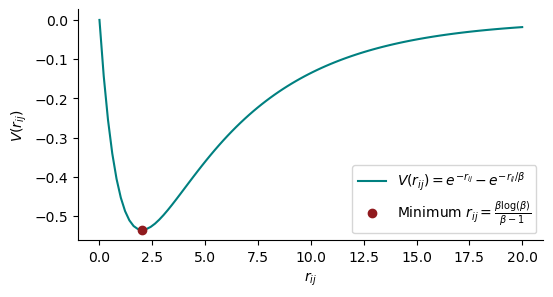
\includegraphics[width=0.6\linewidth]{chapters/Theory/figures/potential.png}
    \caption{The potential well our point particles lie in, with the minimum (ie. effective cell size) drawn in.}
    \label{fig:potential}
\end{figure}
each timestep the cells move as subjects to overdamped dynamics:

\begin{equation}
    \frac{d \bar{x}_i}{d t}=-\frac{d V_i}{d \bar{x}_i}+\eta \hspace{1.5cm}|\hspace{1.5cm}  \bar{x} \in \{\bar{r}, \bar{p}, \bar{q}\}
\end{equation}

where $\eta$ is uncorrelated Gaussian noise.
$\cdots$
Now, just like nature, we will want to break some symmetries for interesting morphologies to emerge.\\
The principal idea is to elevate the Apical-Basal and Planar-Cell polarities by seeing them as explicitly stated polarization vectors with rules for self- and neighbor interaction (mechanotransduction as described in section \ref{sec:theory-polarity})
 introducing a more complicated parameter, A
\begin{equation}
    A_{ij}=\sum_{n=1}^{3}\lambda_n A_n
\end{equation}

\footnote{some iterations of the model keep the constraint $\sum_{n=1}^{3}\lambda_n=1$} 

As previously mentioned the interplay between cell-polarisation and physical orientation goes both ways. This motivates the following three terms which I will quickly explain one by one:
\begin{subequations}
\begin{align}
S_1&=\left(\hat{p}_i \times \hat{r}_{i j}\right) \cdot\left(\hat{p}_j \times \hat{r}_{i j}\right)\label{eq:s1}\\
S_2&=\left(\hat{p}_i \times \hat{q}_{i}\right) \cdot\left(\hat{p}_j \times \hat{q}_{j}\right)\label{eq:s2}\\
S_3&=\left(\hat{q}_i \times \hat{r}_{i j}\right) \cdot\left(\hat{q}_j \times \hat{r}_{i j}\right)\label{eq:s3}
\end{align}
\end{subequations}

As can be seen, the dot-product of cross products are used multiple times. This configuration can be understood for $\left(a \times b\right) \cdot\left(c \times d\right)$ as "keep a and c and c and d respectively parallel, while keeping a and b perpendicular".\\

$S_1$ (Equation \ref{eq:s1}) makes sheets, keeping the Apical and Basal sides of the cells parallel, but also perpendicular to vector between the cell centers. \\
$S_2$ (\ref{eq:s2}) keeps the Apical-Basal and Planar-Cell-polarities perpendicular within each cell, but aligned across cells.\\
$S_3$ (\ref{eq:s3}), finally, is lowest when the Planar-Cell-polarities are aligned but perpendicular. In the realm where this dominates, the cell sheets created by $S_1$ are exchanged for lines of cells perpendicular to their PCP-vectors. $S_3$ is the main driver of in-plane motion.\\

\begin{figure}[H]
    \centering
    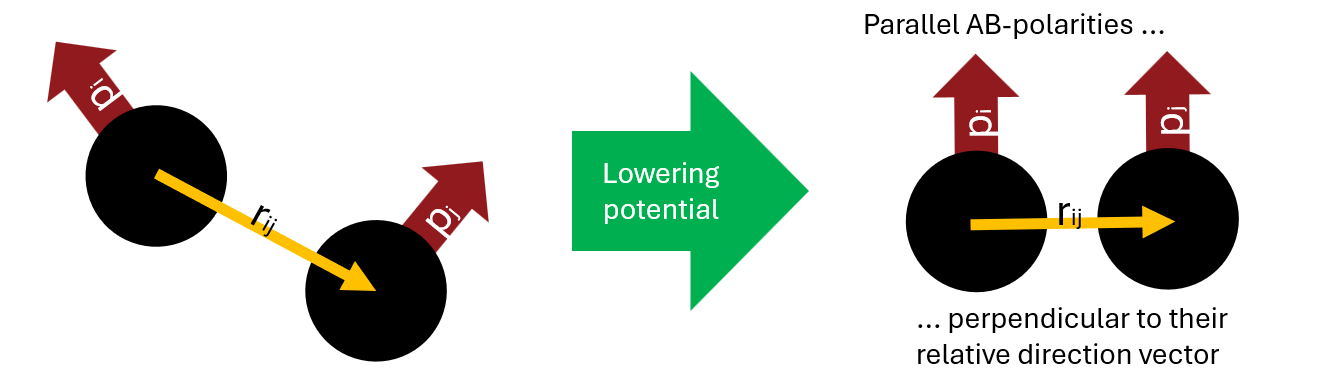
\includegraphics[width=0.3\linewidth]{chapters/Theory/figures/explainS1.png}
    \caption{A visual help for understanding the influence of the $S_1$-term (Equation \ref{eq:s1}). The orange arrow is the AB-polarity and the blue circles representations of the positions of the cells.}
    \label{fig:explain-S1}
\end{figure}

Now, having a potential defined, a number of modifications where added:
\begin{itemize}
    \item Cell types
        \begin{itemize}
            \item As the different domains of the embryo act differently, we need to be able to define different cell types [mainly different $\lambda$-values for different cells.]
        \end{itemize}
    \item Boundary conditions
        \begin{itemize}
            \item A vital part of both the development of the fruit fly and this model is the cells interactions with their boundary conditions. From images of the chorion (egg-shell for you non-biologists) we parameterized the 3-dimensional shape, adding a boundary to the potential. 
        \end{itemize}
    \item Preferential adhesion
        \begin{itemize}
            \item 
        \end{itemize}
    \item Nematic 
    \item Lower apical area when constricting
\end{itemize}


As the model is purely point-based, whenever we speak of inter-cellular junctions, neighbors, areas or angles, everything is extracted from the point cloud and voronoi-neighbors.

\section{Implementation}
The gradient is calculated via an automatic differentiation engine\footnote{The PyTorch-framework specifically} and the simulation time steps are calculated via Euler integration.

This is not interesting to read about, so extensive notes on the actual implementation along with pseudocode, can be found in Section \ref{App:Code} in the Appendix.

